\documentclass[letterpaper]{article}
\usepackage{settings}

\begin{document}
\begin{notes}{Part 3: Features}

\NoteChapter{Objects in Image Processing: Edges, Corners, and Blobs}


\NoteSection{Edges}

\NoteSubsection{What is an Edge?}

An \textbf{edge} is a location where intensity changes abruptly. Physically, edges arise from:
\begin{itemize}
    \item \emph{Depth discontinuity}: objects at different distances occlude one another
    \item \emph{Surface orientation discontinuity}: adjacent surfaces with different normals reflect light differently
    \item \emph{Reflectance discontinuity}: material or color change at an object boundary
    \item \emph{Illumination discontinuity}: cast shadows create sharp intensity boundaries
\end{itemize}

\begin{figure}[H]
    \centering
    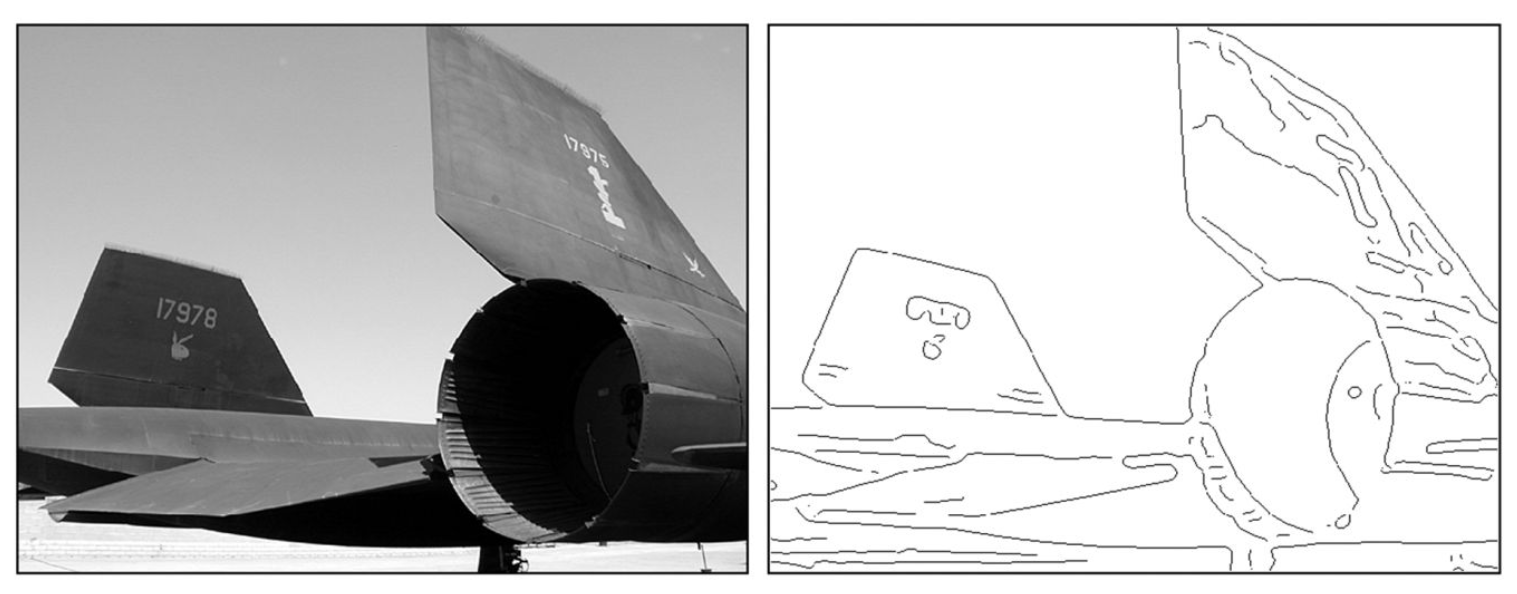
\includegraphics[width=0.85\linewidth]{images/part3/edge-visualized.png}
    \caption{Visualization of Edges}
\end{figure}

\textbf{Edge models.} Idealised 1D profiles perpendicular to the edge:
\begin{itemize}
    \item \emph{Step edge}: intensity jumps instantaneously. First derivative is a spike; second derivative has a zero-crossing.
    \item \emph{Ramp edge}: intensity changes linearly over several pixels (blurred step). First derivative is a plateau.
    \item \emph{Roof/ridge edge}: intensity rises then falls - thin bright or dark line. Second derivative has two zero-crossings.
\end{itemize}
First-derivative operators (Sobel, Prewitt) detect step edges via large gradient magnitude. Second-derivative operators (Laplacian, LoG) detect edges via zero-crossings.

\NoteSubsection{Derivative Models for Basic Edge Detection}

\textbf{1D analysis.} For a continuous 1D signal $f(x)$, a step edge appears as:
\begin{itemize}
    \item a \emph{peak} in $|f'(x)|$ - the first derivative has maximum magnitude at the transition
    \item a \emph{zero-crossing} in $f''(x)$ - the second derivative changes sign exactly at the edge
\end{itemize}
Discrete finite-difference approximations on a sampled signal:
\begin{align*}
f'(x) &\approx \tfrac{1}{2}\bigl[f(x+1)-f(x-1)\bigr] && \text{(central difference, 1st order)}\\
f''(x) &\approx f(x+1) - 2f(x) + f(x-1) && \text{(central difference, 2nd order)}
\end{align*}
Two detection strategies follow:
\begin{itemize}
    \item \emph{First-order}: threshold $|f'(x)|$; flag pixels where gradient magnitude exceeds $T$.
    \item \emph{Second-order}: find zero-crossings of $f''(x)$; gives sub-pixel localisation but is sensitive to noise.
\end{itemize}

\textbf{2D gradient.} For an image $f(x,y)$, the gradient vector
$$\nabla f = \begin{bmatrix}f_x \\ f_y\end{bmatrix} = \begin{bmatrix}\partial f/\partial x \\ \partial f/\partial y\end{bmatrix}$$
points in the direction of maximum intensity increase. Its magnitude and direction are
$$|\nabla f| = \sqrt{f_x^2 + f_y^2}, \qquad \theta = \arctan\!\left(\frac{f_y}{f_x}\right).$$
The edge direction is \emph{perpendicular} to $\nabla f$ (i.e.\ the gradient is orthogonal to the edge contour). Practical approximations replace the partial derivatives with finite-difference kernels (Sobel, Prewitt).\\

% \begin{figure}[H]
%     \centering
%     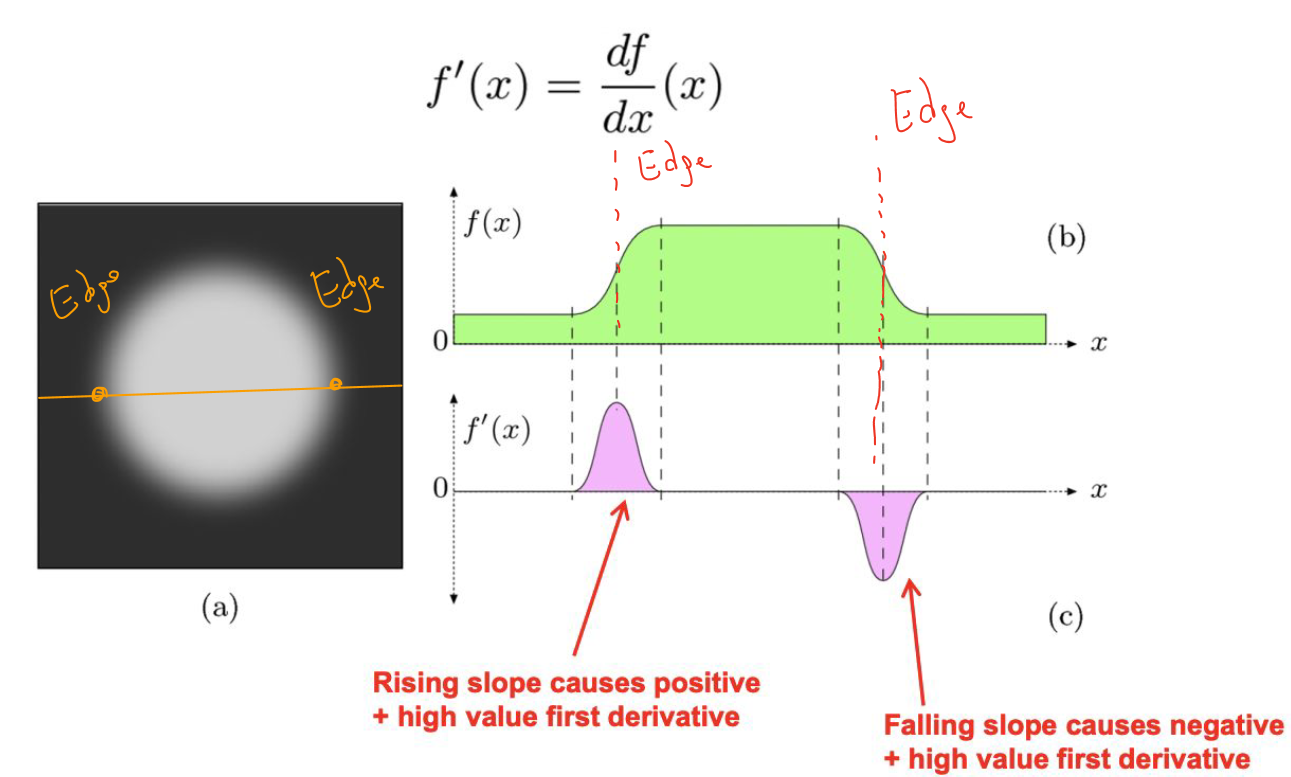
\includegraphics[width=0.9\linewidth]{images/part3/derivative-edge.png}
% \end{figure}


\textbf{2D Laplacian.} The isotropic second-order operator is
$$\nabla^2 f = \frac{\partial^2 f}{\partial x^2} + \frac{\partial^2 f}{\partial y^2} \approx f(x+1,y)+f(x-1,y)+f(x,y+1)+f(x,y-1)-4f(x,y).$$
Edge pixels are located at zero-crossings of $\nabla^2 f$. Because the Laplacian amplifies noise, it is always preceded by Gaussian smoothing (giving the LoG filter).\\

\textbf{Key trade-off.} First-order methods yield gradient direction and are easy to threshold, but produce thick edges requiring NMS. Second-order zero-crossings are precisely localised to single pixels but are noisier - hence the importance of LoG and the Canny pipeline.

\NoteSubsection{Canny Edge Detector (1986)}

The Canny detector is the standard pipeline for thin, well-localised, noise-robust edges. It jointly optimises three criteria: \emph{good detection} (low miss/false-alarm rate), \emph{good localisation} (edges marked close to true boundary), and \emph{single response} (one edge pixel per true edge).\\

\textbf{Algorithm.}
\begin{enumerate}
    \item \textit{Gaussian smoothing.} Convolve with $G_\sigma$ to suppress noise. Larger $\sigma$ reduces noise sensitivity but blurs fine edges.
    \item \textit{Gradient computation.} Compute magnitude $M = \sqrt{G_x^2 + G_y^2}$ and direction $\theta = \arctan(G_y / G_x)$ using Sobel kernels.
    \item \textit{Non-maximum suppression (NMS).} Thin edges to one pixel. Suppress any pixel whose magnitude $M$ is not a local maximum along the gradient direction $\theta$. Result: single-pixel-wide ridges.
    \item \textit{Double thresholding.} Classify surviving pixels with thresholds $T_L < T_H$ (typical ratio $T_H/T_L = 2$--$3$):
    \begin{itemize}
        \item $M \ge T_H$: \emph{strong edge}
        \item $T_L \le M < T_H$: \emph{weak edge}
        \item $M < T_L$: suppressed
    \end{itemize}
    \item \textit{Edge tracking by hysteresis.} Keep a weak edge pixel if and only if it is 8-connected to at least one strong edge pixel. Links genuine contours while discarding isolated noise responses.
\end{enumerate}


\begin{figure}[H]
    \centering
    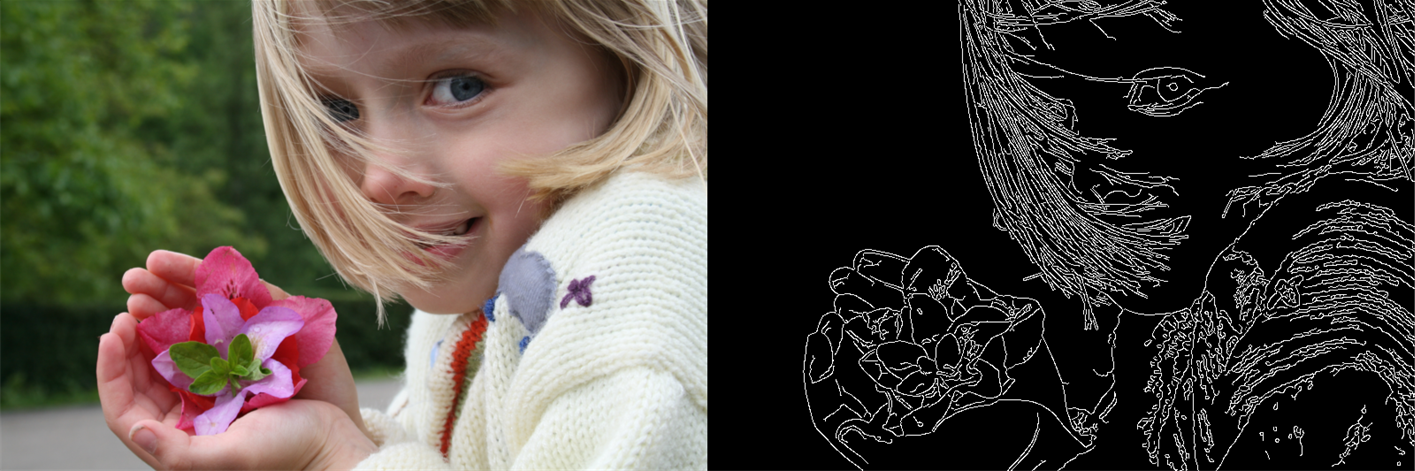
\includegraphics[width=0.9\linewidth]{images/part3/canny-edge.png}
    \caption{Canny Edge detector applied to a photo}
\end{figure}


\NoteSubsection{Difference of Gaussians (DoG)}

DoG approximates the LoG by subtracting two Gaussians at different scales:
$$\mathrm{DoG}_{\sigma_1,\sigma_2}(x,y) = G_{\sigma_1}(x,y) - G_{\sigma_2}(x,y), \quad \sigma_1 < \sigma_2.$$
When $\sigma_2/\sigma_1\approx 1.6$, DoG closely approximates $(\sigma_2^2-\sigma_1^2)\nabla^2 G_\sigma$. Edge locations are zero-crossings of the DoG response. Computationally cheaper than LoG (two Gaussian blurs, no explicit Laplacian kernel). Used as the blob/edge detector in the SIFT feature pipeline.

\begin{figure}[H]
    \centering
    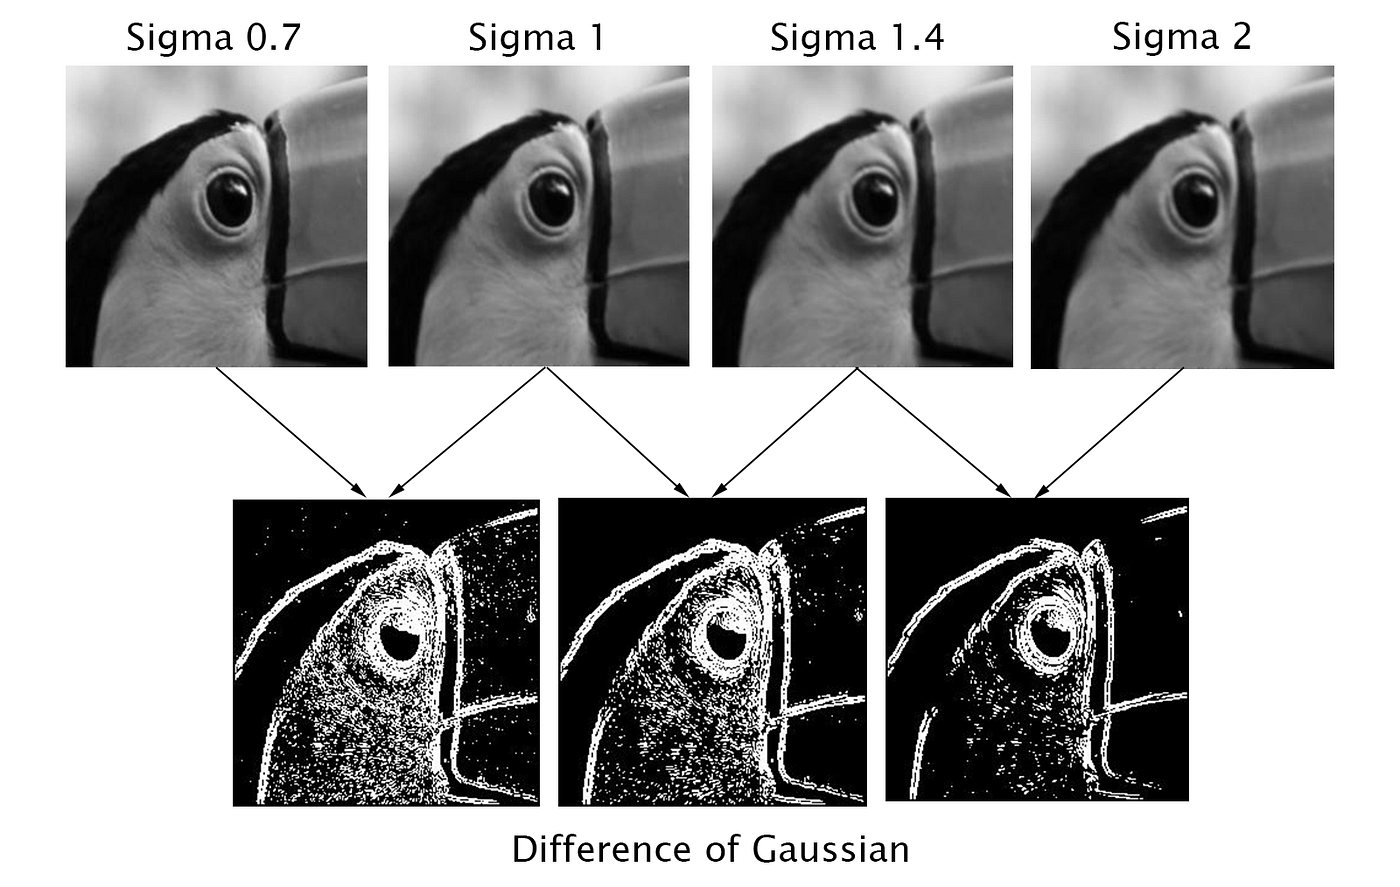
\includegraphics[width=1\linewidth]{images/part3/dog.png}
    \caption{Difference of Gaussian Illustration}
\end{figure}


\columnbreaknofill

\NoteSection{Corners}

\NoteSubsection{Corner Detection}

A \textbf{corner} is a point with large intensity variation in \emph{multiple} directions simultaneously. Unlike edges (localised in only one direction), corners are well-localised in 2D and are repeatable under viewpoint and illumination changes.

\begin{itemize}
    \item Saliency: Corners are found at “interesting” regions of an image.
    \item Localization: Corners occupy a small region: used to pinpoint information.
    \item Repeatability: Photometric or geometric transformations do not affect the corner.
\end{itemize}

\textbf{Flat vs.\ edge vs.\ corner.} Shift a small window $W$ by $(\Delta x, \Delta y)$; the sum of squared differences is
$$E(\Delta x,\Delta y) = \sum_{(x,y)\in W}\bigl[f(x+\Delta x, y+\Delta y) - f(x,y)\bigr]^2.$$
\begin{itemize}
    \item \emph{Flat}: $E$ small for all shift directions
    \item \emph{Edge}: $E$ large only perpendicular to the edge
    \item \emph{Corner}: $E$ large in all directions
\end{itemize}

\begin{figure}[H]
    \centering
    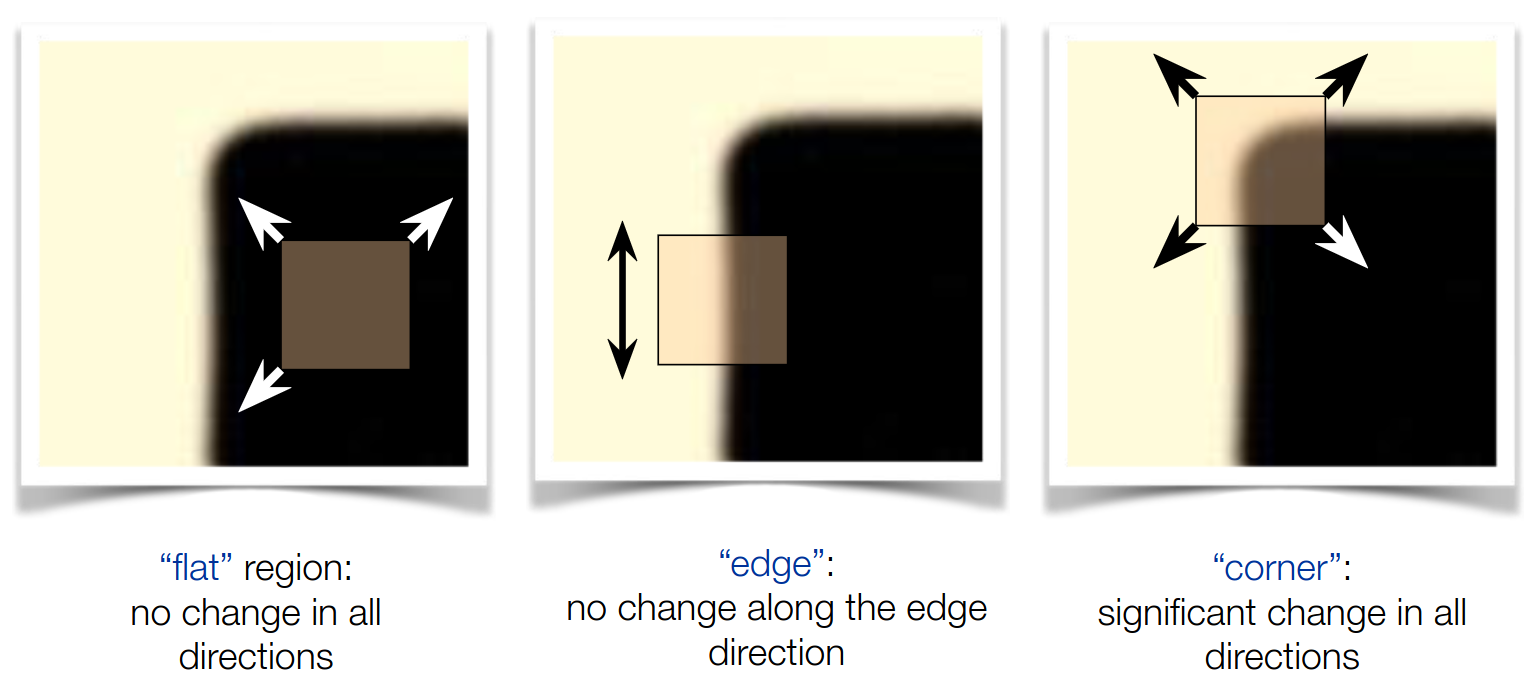
\includegraphics[width=1\linewidth]{images/part3/flat-edge-corner.png}
    \caption{Flat vs.\ edge vs.\ corner.}
\end{figure}


\NoteSubsection{Moravec Corner Detector (1980)}

The earliest interest-point detector (Moravec, 1980). The core idea: a corner is where shifting a small window in \emph{any} direction causes a large intensity change.\\

\textbf{Algorithm.}
\begin{enumerate}
    \item Fix a window $W$ (typically $5\times5$) centred at pixel $(x,y)$.
    \item Compute the SSD for each of four discrete shifts $\Delta \in \{(1,0),(0,1),(1,1),(1,-1)\}$:
    $$\mathrm{SSD}_\Delta(x,y) = \sum_{(s,t)\in W}\bigl[f(x{+}s{+}\Delta x,\,y{+}t{+}\Delta y) - f(x{+}s,\,y{+}t)\bigr]^2.$$
    \item Take the \emph{minimum} over all four shifts as the corner strength:
    $$C(x,y) = \min_{\Delta}\,\mathrm{SSD}_\Delta(x,y).$$
    The minimum captures the weakest direction - a corner must be strong in \emph{every} direction.
    \item Threshold: candidate corner if $C(x,y) > T$.
    \item Non-maximum suppression: keep only local maxima of $C$ in a neighbourhood.
\end{enumerate}

\textbf{Interpretation of $C$.}
\begin{itemize}
    \item $C$ large in all directions $\Rightarrow$ corner
    \item $C$ large only perpendicular to one direction $\Rightarrow$ edge
    \item $C$ small everywhere $\Rightarrow$ flat region
\end{itemize}

\textbf{Limitations.}
\begin{itemize}
    \item Only 4 discrete shift directions - anisotropic; misses edges at intermediate angles.
    \item Uniform (box) window weighting - no noise suppression; pixels near the boundary contribute as much as those at the centre.
    \item Hard threshold on $C$; no smooth response grading.
    \item Not rotation-invariant.
\end{itemize}
Harris addresses all four: the structure tensor $M$ integrates over \emph{all} directions via gradients, the Gaussian window downweights boundary pixels, the response $R$ is continuous, and $M$'s eigenvalues are rotation-invariant.


\NoteSubsection{Harris Corner Detector (1988)}

Harris \& Stephens (1988) fix Moravec's limitations by replacing discrete shifts with a continuous gradient formulation.\\

\textbf{Algorithm.}
\begin{enumerate}
    \item \textit{Compute image gradients.} Compute $f_x = \partial f/\partial x$ and $f_y = \partial f/\partial y$ using Sobel, Prewitt (or similar) kernels.
    \item \textit{Form the structure tensor.} At each pixel, build the outer-product matrix and smooth it with a Gaussian window $G_\sigma$:
    $$M(x,y) = G_\sigma * \begin{bmatrix}f_x^2 & f_x f_y \\ f_x f_y & f_y^2\end{bmatrix}.$$
    This integrates gradient information over a neighbourhood, weighting central pixels more heavily. The Taylor-linearised SSD then satisfies
    $$E(\Delta x,\Delta y) \approx \begin{bmatrix}\Delta x & \Delta y\end{bmatrix} M \begin{bmatrix}\Delta x\\\Delta y\end{bmatrix}.$$
    \item \textit{Classify via eigenvalues.} The eigenvalues $\lambda_1 \ge \lambda_2$ of $M$ describe local geometry:
    \begin{center}
    \begin{tabular}{@{}lll@{}}
    \toprule
    $\lambda_1$ & $\lambda_2$ & Region type \\
    \midrule
    small & small & flat \\
    large & small & edge \\
    large & large & corner \\
    \bottomrule
    \end{tabular}
    \end{center}
    \item \textit{Compute corner response.} To avoid eigendecomposition, use
    $$R = \det(M) - k\,[\mathrm{tr}(M)]^2 = \lambda_1\lambda_2 - k(\lambda_1+\lambda_2)^2, \quad k \approx 0.04\text{--}0.06.$$
    \begin{itemize}
        \item $R \gg 0$: corner (both $\lambda$ large)
        \item $R \ll 0$: edge (one $\lambda$ dominates)
        \item $|R| \approx 0$: flat
    \end{itemize}
    \item \textit{Threshold and NMS.} Keep pixels where $R > T$ and $R$ is a local maximum in a $3\times3$ (or larger) neighbourhood.
\end{enumerate}

\textbf{Properties.} Rotation-invariant (eigenvalues are invariant to rotation of image coordinates). Not scale-invariant - the detected corners change as the image is rescaled.

\NoteSubsection{Shi-Tomasi Corner Detector (1994)}

Shi and Tomasi replace the Harris response with
$$R_{\mathrm{ST}} = \min(\lambda_1, \lambda_2).$$
A pixel is a corner if $\min(\lambda_1,\lambda_2) > \tau$. Both eigenvalues must exceed the threshold, giving more uniformly distributed, stable corners. Used in OpenCV's \texttt{goodFeaturesToTrack}.

\NoteSubsection{Noble Corner Detector (1998)}

Noble replace the Harris response with
$$R_{\mathrm{ST}} = \frac{\det(M)}{\mathrm{trace}(M) + \epsilon}$$
where $\epsilon$ is a small positive constant.


\NoteSubsection{Förstner Corner Detector (1987)}

Förstner \& Gülch (1987) predates Harris and takes a fundamentally different approach: rather than collapsing the structure tensor into a single scalar response, it estimates an \emph{optimal sub-pixel location} for each corner candidate and characterises the uncertainty of that location with an \emph{error ellipse}.\\

\textbf{Motivation.} Each image gradient $\nabla f(x_i, y_i) = (f_{x,i}, f_{y,i})$ defines a constraint line through $(x_i, y_i)$ orthogonal to the gradient: all points along the edge satisfy this line equation. At a true corner, many such lines from different directions meet at a single point. The optimal intersection $\hat{\mathbf{p}} = (\hat{u}, \hat{v})$ minimises the weighted sum of squared perpendicular distances to all gradient lines in a neighborhood $W$:
$$\hat{\mathbf{p}} = \arg\min_{\mathbf{p}} \sum_{(x_i,y_i)\in W} w_i \bigl(f_{x,i}(u-x_i)+f_{y,i}(v-y_i)\bigr)^2.$$
Setting the gradient to zero gives the normal equations $M\hat{\mathbf{p}} = \mathbf{b}$, where $M$ is the (Gaussian-windowed) structure tensor and
$$\mathbf{b} = G_\sigma * \begin{bmatrix}f_x(f_x x + f_y y)\\ f_y(f_x x + f_y y)\end{bmatrix}.$$
The sub-pixel corner estimate is therefore $\hat{\mathbf{p}} = M^{-1}\mathbf{b}$.\\

\textbf{Error ellipse.} The covariance of $\hat{\mathbf{p}}$ (assuming i.i.d.\ gradient noise with variance $\sigma_0^2$) is
$$\Sigma_{\hat{\mathbf{p}}} = \sigma_0^2\,M^{-1}.$$
Its shape is an ellipse whose axes align with the eigenvectors of $M$ and whose semi-axis lengths are proportional to $1/\sqrt{\lambda_i}$. A small, circular ellipse means the corner is well-localised in all directions - the hallmark of a true corner.\\

\textbf{Two quality measures.} With eigenvalues $\lambda_1 \ge \lambda_2$ of $M$:
\begin{itemize}
    \item \textbf{Roundness} $q$ - how circular the error ellipse is:
    $$q = \frac{4\det M}{(\mathrm{tr}\,M)^2} = \frac{4\lambda_1\lambda_2}{(\lambda_1+\lambda_2)^2} \in (0,1].$$
    $q \to 1$: ellipse is nearly circular (good corner); $q \to 0$: highly elongated (edge - uncertain along it).
    \item \textbf{Size} (localization precision) $w$ - the harmonic mean of the eigenvalues:
    $$w = \frac{\det M}{\mathrm{tr}\,M} = \frac{\lambda_1\lambda_2}{\lambda_1+\lambda_2}.$$
    Large $w$: small error ellipse (well-localised); small $w$: large ellipse (flat or noisy region).
\end{itemize}

\textbf{Algorithm.}
\begin{enumerate}
    \item Compute Gaussian-windowed structure tensor $M$ and right-hand side $\mathbf{b}$ at every pixel.
    \item Compute $q$ and $w$ from $M$.
    \item A pixel is a corner candidate if $q > q_0$ (typically $0.5$) \emph{and} $w > w_0$ (data-dependent threshold).
    \item Sub-pixel refinement: compute $\hat{\mathbf{p}} = M^{-1}\mathbf{b}$ at each candidate.
    \item NMS on $w$ to suppress non-maximal candidates.
\end{enumerate}

\textbf{Key distinction from Harris.} Harris fuses roundness and size into a single response $R = \det M - k(\mathrm{tr}\,M)^2$, which can pass the threshold via a large determinant even if the ellipse is elongated ($q$ small). Förstner's two-threshold scheme ($q$ and $w$ independently) avoids false-positives on strong edges, and the sub-pixel estimate $\hat{\mathbf{p}}$ gives localisation accuracy beyond the pixel grid.

\NoteSubsection{The SUSAN Family (1997)}

SUSAN (\textbf{S}mallest \textbf{U}nivalue \textbf{S}egment \textbf{A}ssimilating \textbf{N}ucleus) (Smith \& Brady, 1997) detects edges and corners without computing image derivatives, using only intensity comparisons within a circular mask.\\

\textbf{Core idea: the USAN area.} For each pixel (the \emph{nucleus}) $\mathbf{r_0}$, place a circular mask of radius $\approx 3.4$ pixels (37 pixels). Count how many mask pixels have similar intensity to the nucleus:
$$n(\mathbf{r_0}) = \sum_{\mathbf{r}\in\text{mask}} c(\mathbf{r},\mathbf{r_0}),$$
using the comparison function
$$c(\mathbf{r},\mathbf{r_0}) = e^{-\left(\frac{f(\mathbf{r})-f(\mathbf{r_0})}{t}\right)^{\!6}},$$
where $t$ is the intensity similarity threshold. (A hard binary version $c=\mathbf{1}[|f(\mathbf{r})-f(\mathbf{r_0})|\le t]$ is also common.) The set of similar pixels is the \textbf{USAN}.\\

\textbf{Geometric interpretation of $n$.}
\begin{itemize}
    \item Nucleus in a \emph{flat region}: nearly all mask pixels are similar $\Rightarrow$ $n \approx n_{\max}$ (large)
    \item Nucleus on an \emph{edge}: roughly half the mask crosses the boundary $\Rightarrow$ $n \approx n_{\max}/2$
    \item Nucleus at a \emph{corner}: only a small wedge of the mask is similar $\Rightarrow$ $n \ll n_{\max}/2$ (small)
\end{itemize}

\textbf{Corner response.} Define the geometric threshold $g = 3n_{\max}/4$. Then:
$$R(\mathbf{r_0}) = \begin{cases} g - n(\mathbf{r_0}), & n(\mathbf{r_0}) < g,\\ 0, & \text{otherwise.}\end{cases}$$
$R>0$ only where the USAN is smaller than $g$, i.e.\ at edges and corners. Corners give the largest $R$. Apply NMS to retain local maxima.


\begin{figure}[H]
    \centering
    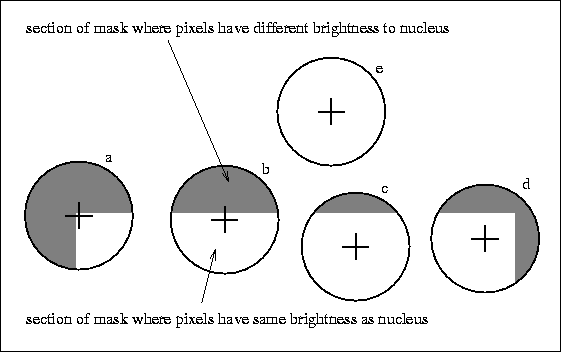
\includegraphics[width=0.85\linewidth]{images/part3/SUSAN.png}
\end{figure}

\textbf{Edge detection with SUSAN.} Edges are where $n \approx n_{\max}/2$. The edge direction is estimated from the centroid of the USAN relative to the nucleus.\\

\textbf{Properties.}
\begin{itemize}
    \item No image derivatives - robust to noise without an explicit smoothing step; $t$ controls sensitivity vs.\ noise.
    \item A single circular mask replaces the rectangular window of Moravec and the gradient kernels of Harris.
    \item Not rotation-invariant (the discrete circular mask breaks symmetry slightly) and not scale-invariant.
    \item Directly inspired FAST: FAST's segment test is a fast approximation of the USAN area, replacing the full 37-pixel count with a 16-pixel ring and a contiguous-arc criterion.
\end{itemize}


\NoteSubsection{The FAST Corner Detector (2006)}

Features from Accelerated Segment Test (Rosten \& Drummond, 2006). Designed for real-time applications where Harris/Shi--Tomasi are too slow. All decisions are intensity comparisons - no gradients, no matrix operations.\\

\textbf{Circle specification.} Consider the 16 pixels $p_1,\ldots,p_{16}$ on a Bresenham circle of radius 3 around centre pixel $p$, labelled clockwise from the top. Their offsets from $p$ are:
$$(-3,0),(-3,1),(-2,2),(-1,3),(0,3),(1,3),(2,2),(3,1),$$
$$(3,0),(3,-1),(2,-2),(1,-3),(0,-3),(-1,-3),(-2,-2),(-3,-1).$$

\textbf{Segment test.} Let $I_p$ be the intensity of $p$ and $t$ a threshold. Each circle pixel $p_i$ is classified as:
\begin{itemize}
    \item \emph{brighter}: $I_{p_i} > I_p + t$
    \item \emph{darker}: $I_{p_i} < I_p - t$
    \item \emph{similar}: otherwise
\end{itemize}
$p$ is declared a corner if there exist $N$ \emph{contiguous} circle pixels all brighter, or all darker, than the respective threshold. Common variants: \textbf{FAST-9} ($N=9$) and \textbf{FAST-12} ($N=12$). FAST-12 is more conservative (fewer detections, higher precision); FAST-9 detects more corners.\\

\textbf{High-speed rejection (FAST-12).} Test only the four cardinal pixels $p_1, p_5, p_9, p_{13}$ (spaced 90° apart). For 12 contiguous pixels to exist, at least 3 of these 4 must all be brighter or all darker. If this condition fails, $p$ is immediately rejected - at most 4 memory accesses. This pre-test eliminates $\approx$75\% of pixels in typical images.\\

\textbf{Corner score and NMS.} After the segment test, assign a score
$$V(p) = \max\!\left(\;\sum_{p_i \in S_b}(I_{p_i} - I_p - t),\;\sum_{p_i \in S_d}(I_p - I_{p_i} - t)\;\right),$$
where $S_b$ (resp.\ $S_d$) is the set of brighter (resp.\ darker) arc pixels. Retain only local maxima of $V$ - adjacent corners collapse to the single strongest response.

\textbf{Properties.}
\begin{itemize}
    \item No gradient computation, no matrix inversion - extremely fast; suitable for real-time SLAM, tracking, and mobile AR.
    \item Not rotation-invariant (circle is fixed; no orientation assigned). \textbf{ORB} extends FAST by adding an orientation via the intensity centroid method and pairing it with a rotated BRIEF descriptor.
    \item Not scale-invariant - run at multiple scales (image pyramid) to gain partial scale robustness.
    \item Sensitive to noise: no smoothing step. Tuning $t$ balances sensitivity vs.\ false positives.
\end{itemize}

\begin{center}
\begin{tabular}{@{}lcccc@{}}
\toprule
Detector & Year & Rotation inv. & Scale inv. & Speed \\
\midrule
Moravec   & 1980 & No  & No & Fast \\
Harris    & 1988 & Yes & No & Moderate \\
Shi--Tomasi & 1994 & Yes & No & Moderate \\
FAST      & 2006 & No  & No & Very fast \\
\bottomrule
\end{tabular}
\end{center}


\NoteSection{Blobs}

A \textbf{blob} is a connected image region whose intensity (or color) is approximately uniform and differs from its surroundings. Unlike edges (1D features) or corners (0D point features), blobs are 2D structures characterised by both \emph{position} and \emph{scale}. The central challenge is detecting blobs across a range of sizes without prior knowledge of which scale to look at.


\begin{figure}[H]
    \centering
    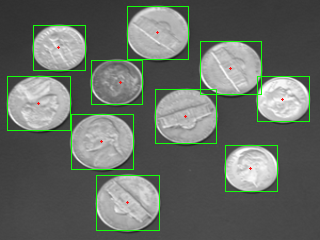
\includegraphics[width=0.6\linewidth]{images/part3/blobs-illustration.png}
\end{figure}

\NoteSubsection{Scale-Space and Characteristic Scale}

\textbf{Scale-space.} Convolving an image $f$ with a Gaussian of width $\sigma$ gives the linear scale-space:
$$L(x,y;\sigma) = G_\sigma(x,y) * f(x,y).$$
Increasing $\sigma$ progressively suppresses fine detail while leaving coarser structure intact. The full set $\{L(\cdot;\sigma)\}_{\sigma>0}$ is the \emph{Gaussian scale-space} of $f$.\\

\textbf{Why the (scale-normalised) LoG?} The Laplacian $\nabla^2 L$ measures how much a pixel differs from its neighborhood - large for blob centers, near zero on flat regions. However, raw LoG responses shrink as $\sigma$ grows (the Gaussian spreads and flattens). To compare responses across scales fairly, multiply by $\sigma^2$:
$$\mathcal{L}(x,y;\sigma) = \sigma^2\,\nabla^2 L(x,y;\sigma) = \sigma^2\bigl(\nabla^2 G_\sigma\bigr)*f(x,y).$$
This is the \emph{scale-normalised LoG} (Lindeberg, 1994). For a bright circular blob of radius $r$, $\mathcal{L}$ peaks at the \emph{characteristic scale}:
$$\sigma^* = \frac{r}{\sqrt{2}},$$
so the blob radius can be read off as $r = \sigma^*\sqrt{2}$. Detecting blobs therefore reduces to finding local extrema of $\mathcal{L}$ jointly over space \emph{and} scale.

\begin{figure}[H]
    \centering
    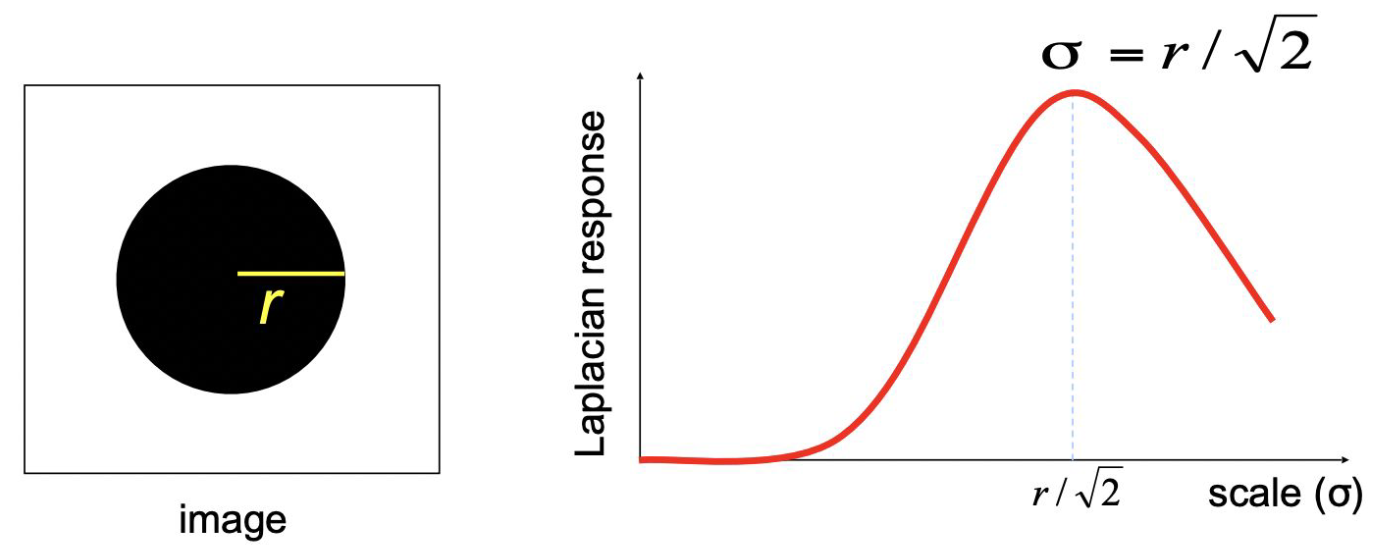
\includegraphics[width=0.8\linewidth]{images/part3/scaled-log.png}
\end{figure}



\NoteSubsection{LoG Blob Detector}

\textbf{Algorithm.}
\begin{enumerate}
    \item Build a discrete scale-space by computing $L(\cdot;\sigma_k)$ for $k = 1,\dots,K$ (typically spaced by a factor of $\sqrt{2}$ or $2$).
    \item At each scale compute the scale-normalised LoG: $\mathcal{L}(x,y;\sigma_k) = \sigma_k^2\,\nabla^2 G_{\sigma_k} * f$.
    \item Detect \emph{local extrema} in the 3D volume $(x,y,\sigma)$: a pixel is a blob candidate if $\mathcal{L}$ is larger (or smaller) than all 26 neighbors - its $3\times3$ spatial neighborhood at the same scale \emph{and} the corresponding $3\times3$ patches at the adjacent scales.
    \item Threshold to suppress weak responses; NMS to retain strongest detections.
\end{enumerate}

The result is a set of circles $(x_i, y_i, r_i)$ - position and estimated radius - that are scale-covariant: if the image is rescaled by a factor $s$, the detected radii scale by the same $s$.

\NoteSubsection{Difference of Gaussians (DoG) Blob Detector}

DoG approximates the scale-normalised LoG and is the basis of SIFT blob detection.\\

\textbf{Approximation.} For adjacent scales $\sigma$ and $k\sigma$ (with $k > 1$ close to 1):
$$G_{k\sigma} - G_\sigma \;\approx\; (k-1)\,\sigma\,\frac{\partial G_\sigma}{\partial\sigma} = (k-1)\,\sigma^2\,\nabla^2 G_\sigma,$$
so
$$\mathrm{DoG}(x,y;\sigma) = L(x,y;k\sigma) - L(x,y;\sigma) \;\approx\; (k-1)\,\mathcal{L}(x,y;\sigma).$$
The constant $(k-1)$ is irrelevant for locating extrema. With $k = 2^{1/s}$ ($s$ intervals per octave), SIFT typically uses $s=3$, computing $s+3$ blurred images per octave (and $s+2$ DoG images), then detecting extrema across $s$ interior DoG scales per octave.\\

\textbf{Scale-space pyramid.}
\begin{enumerate}
    \item Convolve $f$ with Gaussians $G_{\sigma}, G_{k\sigma}, G_{k^2\sigma},\ldots$ (one octave).
    \item Subtract adjacent pairs to get DoG images.
    \item Detect local extrema in the DoG stack as above.
    \item Downsample by $2\times$ to start the next octave.
\end{enumerate}
Two Gaussian blurs and one subtraction replace one Laplacian convolution, at roughly the same cost; the pyramid additionally provides free multi-scale coverage.

\NoteSubsection{Hessian-Based Blob Detection}

\textbf{The Hessian matrix} at scale $\sigma$ captures second-order intensity structure:
$$\mathbf{H}(x,y;\sigma) = \sigma^2\begin{bmatrix} L_{xx} & L_{xy} \\ L_{xy} & L_{yy} \end{bmatrix},$$
where $L_{xx} = \partial^2 L/\partial x^2$, etc.\ (scale-normalised second derivatives). For a circular blob:
\begin{itemize}
    \item $\det(\mathbf{H}) = \sigma^4(L_{xx}L_{yy} - L_{xy}^2)$ is maximised at the blob center and characteristic scale. Used in \textbf{SURF} (Bay et al., 2006).
    \item $\mathrm{tr}(\mathbf{H}) = \sigma^2(L_{xx}+L_{yy}) = \mathcal{L}$ - the LoG. The trace and determinant share the same extrema for isotropic blobs.
\end{itemize}

\textbf{SURF} (Speeded Up Robust Features) approximates the Gaussian second derivatives $L_{xx}$, $L_{yy}$, $L_{xy}$ with box filters, enabling $O(1)$ evaluation via \emph{integral images}:
$$II(x,y) = \sum_{x'\le x,\,y'\le y} f(x',y').$$
Any rectangular sum is computed in 4 table lookups. Box-filter approximations allow SURF to evaluate the Hessian determinant at any scale and position in constant time, making it significantly faster than LoG or DoG.

\NoteSubsection{Maximally Stable Extremal Regions (MSER)}

MSER (Matas et al., 2004) detects blob-like regions without any Gaussian filtering, using only intensity thresholding.\\

\textbf{Extremal regions.} For a threshold $t$, the set $\mathcal{R}(t) = \{(x,y): f(x,y) \le t\}$ is thresholded; each connected component of $\mathcal{R}(t)$ is an \emph{extremal region}. As $t$ increases from $0$ to $L-1$, regions grow and merge (a sequence tracked efficiently by union-find).\\

\textbf{Stability criterion.} A region $\mathcal{R}(t)$ is \emph{maximally stable} if its relative area change
$$q(t) = \frac{|\mathcal{R}(t+\Delta) \setminus \mathcal{R}(t-\Delta)|}{|\mathcal{R}(t)|}$$
is a local minimum over $t$. Stable regions are those that persist over a wide range of thresholds - they correspond to distinctly darker (or lighter) blobs with clear boundaries.\\

\textbf{Properties.}
\begin{itemize}
    \item Invariant to monotone intensity transformations (re-thresholding gives the same regions).
    \item \emph{Affine covariant}, not just similarity covariant - MSER shapes are fit with ellipses and normalised to a canonical circular patch, enabling wide-baseline matching across significant viewpoint change.
    \item No smoothing step; very fast (near-linear in pixels).
    \item Fails on textured or blurry boundaries where no stable threshold exists.
\end{itemize}

\begin{center}
\begin{tabular}{@{}lcccc@{}}
\toprule
Detector & Basis & Scale inv. & Speed \\
\midrule
LoG       & Scale-norm.\ Laplacian & Yes & Slow \\
DoG (SIFT) & Gaussian subtraction & Yes & Moderate \\
SURF      & Box-filter Hessian & Yes & Fast \\
MSER      & Threshold sweep & Yes (affine) & Fast \\
\bottomrule
\end{tabular}
\end{center}


\columnbreaknofill



\NoteChapter{Features}


\NoteSection{Feature Pipeline}

A \textbf{feature} is a compact, meaningful representation of local image structure that can be reliably detected and matched across different images of the same scene. Features bridge raw pixels and high-level tasks such as object recognition, 3D reconstruction, and image retrieval.

\begin{figure}[H]
    \centering
    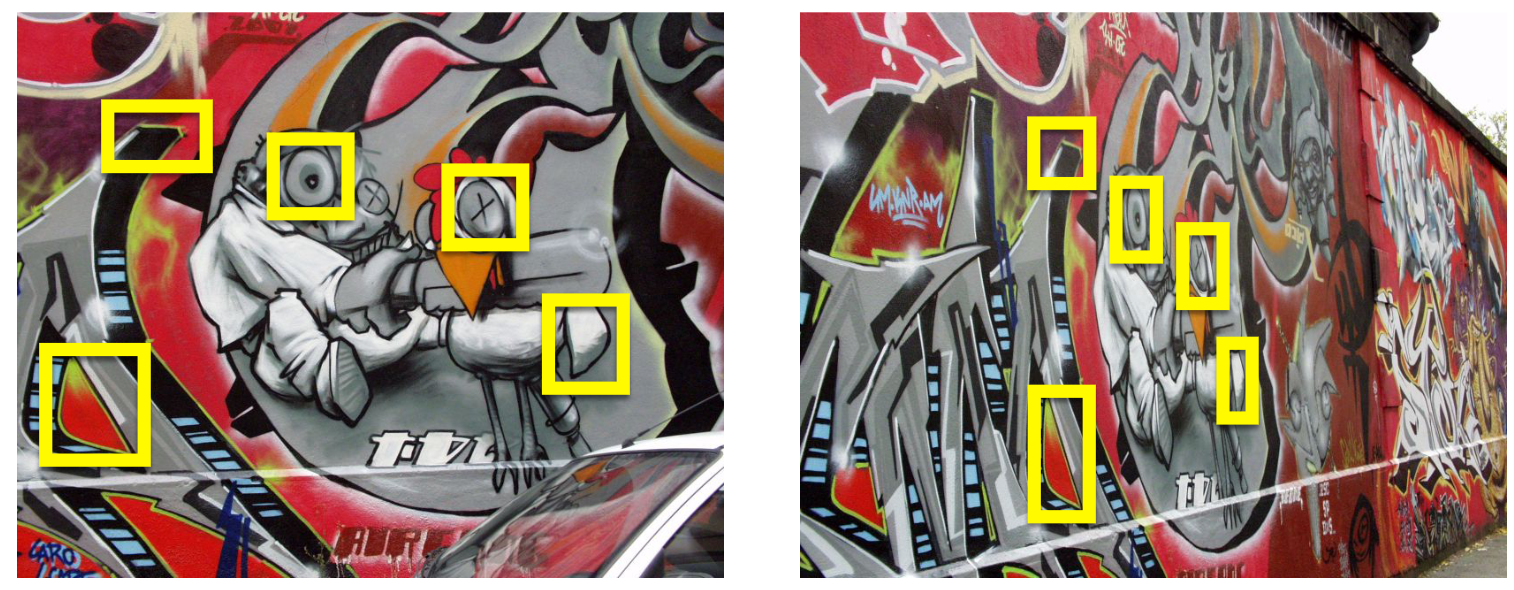
\includegraphics[width=1\linewidth]{images/part3/features-demo.png}
\end{figure}

A complete feature pipeline has three stages:
\begin{itemize}
    \item \textbf{Detector} - locates \emph{where} interesting structure exists (position, scale, orientation). A good detector is \emph{repeatable}: it fires at the same physical scene point across different images. Flat regions and edges are poor candidates; corners and blobs are preferred because they are localised in multiple directions (see CORNERS and BLOBS).
    \item \textbf{Descriptor} - encodes \emph{what} the local patch looks like into a fixed-length vector or bit string. It must be \emph{distinctive} (different points $\to$ different vectors) and \emph{invariant} (the same point under different conditions $\to$ the same vector).
    \item \textbf{Matcher} - establishes correspondences by comparing descriptors, then uses geometric verification (e.g.\ RANSAC) to filter outliers.
\end{itemize}

\textbf{Desiderata.} Repeatability (detector fires at the same scene point despite appearance change); distinctiveness (correct match much closer in descriptor space than any incorrect one); locality (small patch $\Rightarrow$ robust to occlusion); sufficient quantity and computational efficiency for the application.\\

\textbf{Invariance vs.\ discriminability.} Baking invariance to a transformation into a descriptor always discards information - the art is choosing which invariances matter (scale, rotation, illumination) while preserving enough structure to remain discriminative.\\

\textbf{Taxonomy of this section.}
\begin{enumerate}
    \item \emph{Local keypoint pipelines} (SIFT, SURF, binary): detect sparse interest points; describe each with a local patch vector.
    \item \emph{Dense descriptors} (HOG): compute descriptors on a regular grid over a detection window, not at sparse keypoints - used for classification and detection.
    \item \emph{Matching and geometric verification}: compare descriptor sets across images; filter with ratio test and RANSAC.
    \item \emph{Image-level aggregation} (BoW, VLAD, Fisher): encode an entire image's descriptor set into one fixed-length vector for retrieval and classification.
\end{enumerate}


\NoteSection{RANSAC}

\textbf{RANdom SAmple Consensus} (RANSAC, Fischler \& Bolles 1981) is a general-purpose iterative algorithm for robustly fitting a parametric model to data that contains a large fraction of \emph{outliers} - observations that do not conform to the model. Classical estimators such as least squares are \emph{non-robust}: a single outlier can arbitrarily corrupt the solution. RANSAC instead searches for the model supported by the \emph{largest consistent subset} of the data, tolerating outlier fractions $e$ well above 50\%.\\

\NoteSubsection{Generic RANSAC}

\textbf{Motivating example.} Suppose you have 100 2D points that roughly lie on a straight line, but 60 of them are random noise (outliers). Least squares fits the line to \emph{all} 100 points and gets pulled toward the noise. RANSAC instead asks: \emph{``which line has the most points near it?''} It tries many candidate lines, each built from a tiny random sample, and picks the winner.

\begin{figure}[H]
    \centering
    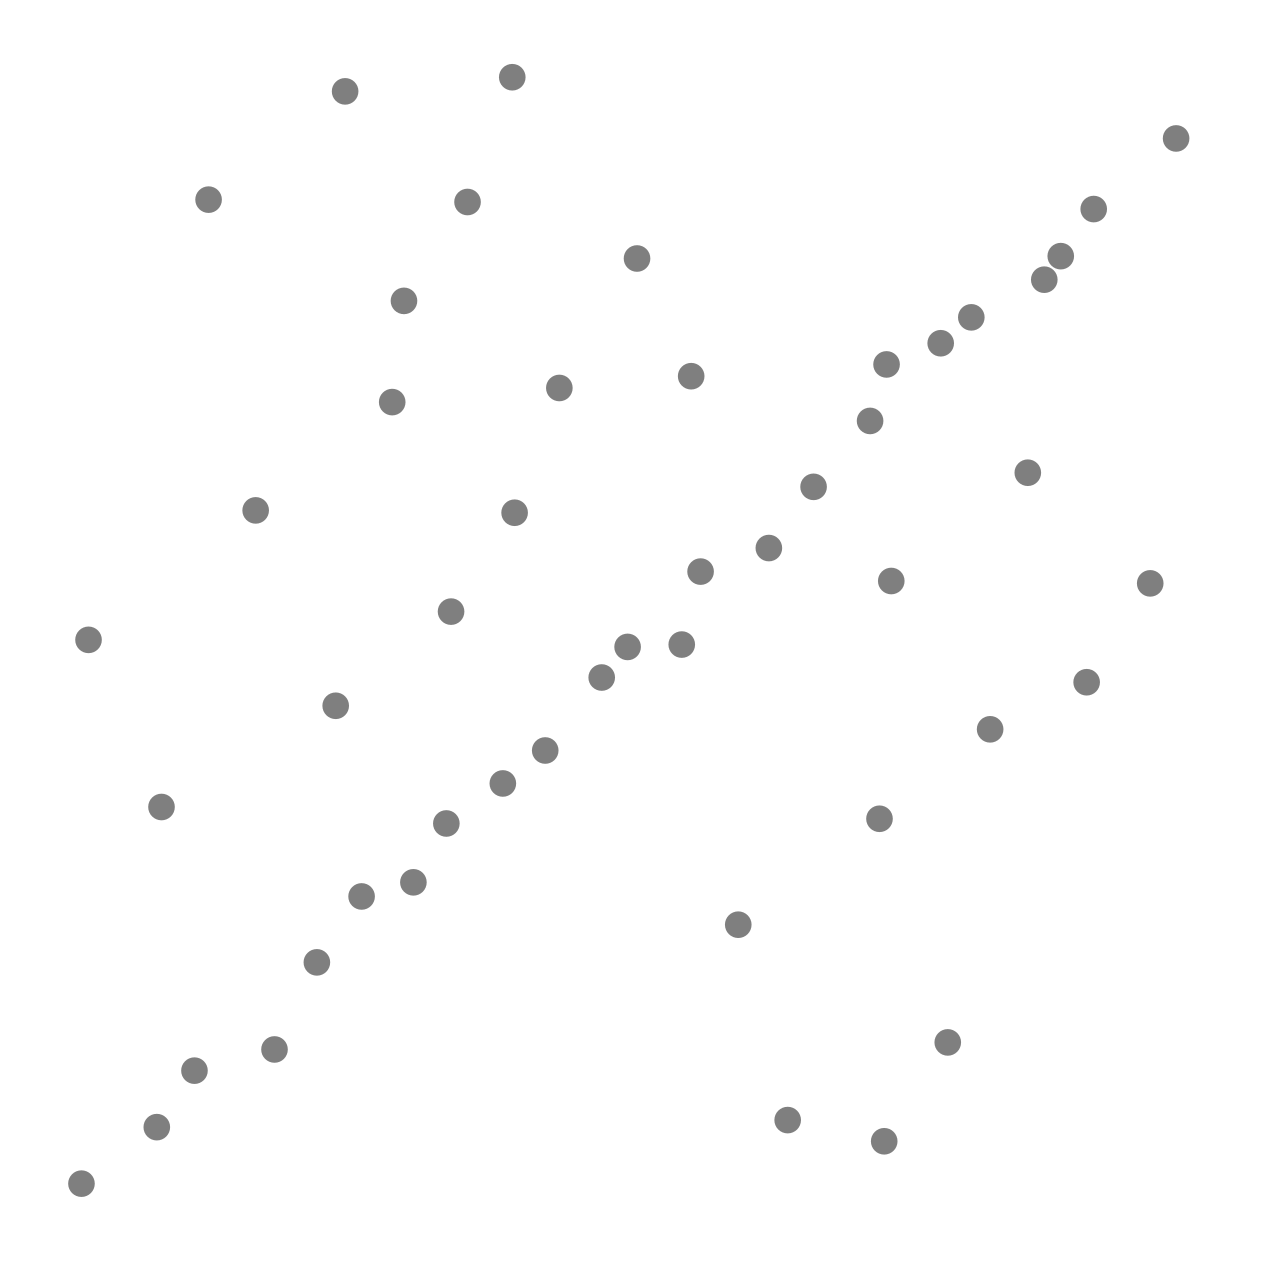
\includegraphics[width=0.4\linewidth]{images/part3/lots-of-points.png}
\end{figure}


\textbf{Parametric model family.} A \emph{parametric model} is any mathematical structure described by a fixed set of numbers (parameters) $\boldsymbol{\theta}$. The model family $\mathcal{M}(\boldsymbol{\theta})$ is the collection of all possible instances as $\boldsymbol{\theta}$ varies:
\begin{itemize}
    \item A 2D line $ax + by + c = 0$ has parameters $\boldsymbol{\theta} = (a,b,c)$.
    \item A circle $(x-h)^2+(y-k)^2=r^2$ has parameters $\boldsymbol{\theta} = (h,k,r)$.
    \item A 2D affine transform has 6 parameters; a homography has 8 (up to scale).
\end{itemize}
The model family fixes the \emph{shape} of what you are fitting; the parameters pin down the specific instance.\\

\textbf{Residual function.} The residual $\rho(p_i, \boldsymbol{\theta})$ measures \emph{how far} a data point $p_i$ is from the model $\mathcal{M}(\boldsymbol{\theta})$ - i.e.\ how badly it violates the model. A small residual means $p_i$ is consistent with $\boldsymbol{\theta}$; a large residual means it is an outlier. The exact form depends on the model:
\begin{itemize}
    \item \emph{Line:} perpendicular (point-to-line) distance.
    \[
    \frac{|ax_0 + by_0 + c|}{\sqrt{a^2 + b^2}}
    \]
    
    \item \emph{Circle:} $\bigl|\,\sqrt{(x_i-h)^2+(y_i-k)^2} - r\,\bigr|$ (how far the point is from the circle boundary).
    \item \emph{Homography:} pixel reprojection error $\|\mathbf{x}_i' - H\mathbf{x}_i\|$ (how far the predicted location is from the observed one).
\end{itemize}

\textbf{Inlier threshold $\epsilon$.} A point $p_i$ is declared an \emph{inlier} if $\rho(p_i,\boldsymbol{\theta}) < \epsilon$ - its residual is small enough to plausibly arise from measurement noise rather than the point being wrong. Choosing $\epsilon$ is the main tuning knob: too tight and genuine matches are rejected; too loose and outliers are accepted. A principled choice is $\epsilon \approx 2.5\sigma$ where $\sigma$ is the expected noise standard deviation (covers 95\% of the Gaussian tail).\\

\textbf{Minimum sample size $s$.} Every model requires a minimum number of points to be determined uniquely. Fewer than $s$ points leave the model underdetermined; exactly $s$ gives a unique solution (or finitely many). RANSAC always draws exactly $s$ points per hypothesis to keep each trial as fast as possible and to minimise the chance of including an outlier.\\

\textbf{Algorithm.}
\begin{enumerate}
    \item \textbf{Sample.} Draw $s$ points uniformly at random from $\mathcal{D} = \{p_i\}_{i=1}^n$ (without replacement).
    \item \textbf{Fit.} Solve for parameters $\hat{\boldsymbol{\theta}}$ using only those $s$ points.
    \item \textbf{Score.} Count all data points whose residual falls below $\epsilon$ - these are the inliers for this hypothesis:
    $$\mathcal{I}(\hat{\boldsymbol{\theta}}) = \bigl\{\,i : \rho(p_i,\,\hat{\boldsymbol{\theta}}) < \epsilon\,\bigr\}.$$
    \item \textbf{Iterate.} Repeat steps 1–3 for $k$ iterations; keep the hypothesis $\boldsymbol{\theta}^*$ with the largest inlier count $|\mathcal{I}|$.
    \item \textbf{Refit.} Re-estimate $\boldsymbol{\theta}^*$ using \emph{all} inliers $\mathcal{I}(\boldsymbol{\theta}^*)$ via least squares. Because inliers are (mostly) noise-free true points, this final fit is far more accurate than any single $s$-point hypothesis.
\end{enumerate}

\textbf{Number of iterations.} Each trial succeeds (all $s$ drawn points are inliers) with probability $(1-e)^s$, where $e$ is the outlier fraction. The probability that at least one of $k$ independent trials succeeds is $1-(1-(1-e)^s)^k$. Setting this equal to $p$:
$$k = \frac{\log(1-p)}{\log\bigl(1-(1-e)^s\bigr)}.$$
Since $e$ is unknown, it is estimated adaptively: after each iteration, $e \leftarrow 1 - |\mathcal{I}^*|/n$ and $k$ is updated, enabling early termination as soon as a good hypothesis is found.\\

\textbf{Examples (model / $s$ / residual).}
\begin{itemize}
    \item \emph{2D line} ($s=2$): perpendicular point-to-line distance.
    \item \emph{Circle} ($s=3$): distance from point to circle boundary.
    \item \emph{3D plane} ($s=3$): point-to-plane distance (LiDAR ground removal).
    \item \emph{Homography / affine / fundamental matrix}: transfer error in pixels - see below.
\end{itemize}

\textbf{Properties and limitations.}
\begin{itemize}
    \item \emph{Probabilistic guarantee:} succeeds with probability $\ge p$; outcomes vary across runs.
    \item \emph{Iteration cost:} $k$ grows exponentially with $e$ and $s$. For the fundamental matrix ($s=8$) at $e=0.6$, $p=0.99$, this exceeds $10^4$ iterations.
    \item \emph{Degenerate samples:} some $s$-point draws are geometrically degenerate (e.g.\ three collinear points cannot determine a unique homography). Discard and resample.
\end{itemize}

\NoteSubsection{RANSAC for Geometric Verification (Features)}

In the feature-matching pipeline, raw descriptor matches contain many \emph{outliers} (incorrect correspondences). RANSAC robustly estimates a geometric model - homography $H$, affine $A$, or fundamental matrix $F$ - from noisy correspondences $\{(\mathbf{x}_i, \mathbf{x}_i')\}$. Here data points are correspondence pairs, the model is a transform matrix, and the residual is a \emph{transfer error} in pixel space.\\

\textbf{Algorithm (feature-specific instantiation).}
\begin{enumerate}
    \item \textbf{Sample.} Randomly draw the minimal set of correspondences: $s=3$ (affine), $s=4$ (homography), $s=8$ (fundamental matrix).
    \item \textbf{Fit.} Estimate $M$ from the sample via DLT or the normal equations.
    \item \textbf{Score.} Count inliers with transfer error $d(\mathbf{x}_i', M\mathbf{x}_i) < \epsilon$ (typically $\epsilon = 3$–$5$ px).
    \item \textbf{Iterate} for $k$ iterations; keep $M^*$ with the most inliers.
    \item \textbf{Refit} $M^*$ to all inliers $\mathcal{I}(M^*)$ via least squares.
\end{enumerate}

\textbf{Transfer error metrics.}
\begin{itemize}
    \item \emph{Symmetric reprojection error} (homography): $d = d(\mathbf{x}',H\mathbf{x})^2 + d(\mathbf{x},H^{-1}\mathbf{x}')^2$.
    \item \emph{Sampson distance} (fundamental matrix): first-order approximation to geometric reprojection error, cheaper than the exact epipolar distance.
\end{itemize}

Typical iteration counts for $e=0.5$, $p=0.99$:

\begin{center}
\begin{tabular}{lcc}
\hline
\textbf{Model} & \textbf{Min.\ sample} $s$ & \textbf{Iterations} $k$ \\
\hline
Line (2D) & 2 & 17 \\
Affine & 3 & 35 \\
Homography & 4 & 72 \\
Fundamental matrix & 8 & 1177 \\
\hline
\end{tabular}
\end{center}

\textbf{Notable variants.}
\begin{itemize}
    \item \textbf{MSAC} (Torr \& Zisserman 2000): truncated $\ell_2$ loss instead of binary inlier count - weights near-inliers more gracefully.
    \item \textbf{MLESAC} (Torr \& Zisserman 2000): maximises likelihood under an inlier-Gaussian / outlier-uniform mixture (EM on the inlier set).
    \item \textbf{PROSAC} (Chum \& Matas 2005): samples progressively from the most confident matches (ranked by descriptor distance), reducing iterations by orders of magnitude.
    \item \textbf{LO-RANSAC} (Chum et al.\ 2003): after each best hypothesis, runs a local optimisation on the inlier set before the global update, greatly improving solution quality.
\end{itemize}



\columnbreaknofill

\NoteChapter{Feature Detection Algorithms}

\NoteSection{SIFT (Lowe, 1999/2004)}

\textbf{Scale-Invariant Feature Transform} is the canonical local feature pipeline. It is invariant to scale, rotation, and moderate affine distortion, and robust to illumination change. The algorithm has four stages.

\begin{enumerate}
    \item \textbf{Scale-space extrema detection.}

    Build a Gaussian scale-space by convolving the image with Gaussians at increasing $\sigma$:
    $$L(x,y,\sigma) = G(x,y,\sigma) * I(x,y), \qquad G(x,y,\sigma) = \frac{1}{2\pi\sigma^2}e^{-(x^2+y^2)/(2\sigma^2)}.$$
    Group scales into \emph{octaves}: within each octave use $s$ intervals, so the scale ratio between adjacent levels is $k = 2^{1/s}$ (Lowe uses $s=3$). The base scale of each octave is $\sigma_0 = 1.6$ (at the first octave; the image is upsampled $2\times$ before the first octave in the reference implementation). Compute the \textit{Difference of Gaussians} (DoGs):
    $$D(x,y,\sigma) = L(x,y,k\sigma) - L(x,y,\sigma) \approx (k-1)\,\sigma^2\nabla^2 L.$$
    Each octave produces $s+3$ smoothed images and $s+2$ DoG images; extrema are detected in the $s$ interior DoG scales (leaving one margin on each side for neighbor comparison). A pixel is a candidate if $D(x,y,\sigma)$ is larger (or smaller) than all 26 neighbors in the $3\times3\times3$ $(x,y,\sigma)$ volume.

    \begin{figure}[H]
        \centering
        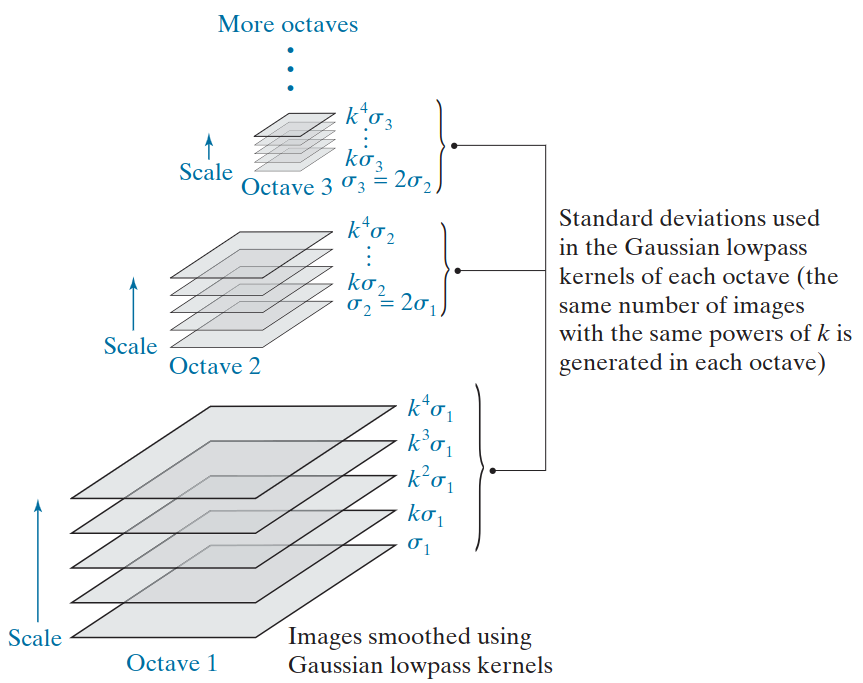
\includegraphics[width=0.75\linewidth]{images/part3/octaves.png}
    \end{figure}

    \item \textbf{Keypoint localisation (sub-pixel / sub-scale).}

    Fit a 3D quadratic to $D$ near each candidate by Taylor expansion about the candidate location $\mathbf{x}_0 = (x,y,\sigma)^T$:
    $$D(\mathbf{x}_0 + \hat{\mathbf{x}}) \approx D(\mathbf{x}_0) + \frac{\partial D}{\partial \mathbf{x}}^T\hat{\mathbf{x}} + \frac{1}{2}\hat{\mathbf{x}}^T \frac{\partial^2 D}{\partial \mathbf{x}^2}\hat{\mathbf{x}}.$$
    Setting the derivative to zero gives the interpolated offset:
    $$\hat{\mathbf{x}} = -\left(\frac{\partial^2 D}{\partial \mathbf{x}^2}\right)^{-1} \frac{\partial D}{\partial \mathbf{x}}.$$
    The Hessian and gradient are approximated by finite differences, e.g.\
    
    \begin{align*}
        \frac{\partial D}{\partial x} &\approx \frac{D(x{+}1,y,\sigma)-D(x{-}1,y,\sigma)}{2},\\
        \frac{\partial^2 D}{\partial x^2} &\approx D(x{+}1,y,\sigma) - 2D(x,y,\sigma) + D(x{-}1,y,\sigma),
    \end{align*}
    
    
    and similarly for $y$, $\sigma$, and cross-terms. If $|\hat{x}_i| > 0.5$ in any dimension, the candidate is moved to the adjacent sample and the fit is repeated (up to 5 iterations). The interpolated value at the extremum is:
    $$D(\hat{\mathbf{x}}) = D(\mathbf{x}_0) + \frac{1}{2}\frac{\partial D}{\partial \mathbf{x}}^T\hat{\mathbf{x}}.$$

    \begin{enumerate}
        \item \emph{Low-contrast rejection.} Discard if $|D(\hat{\mathbf{x}})| < 0.03$ - the extremum is too weak to be stable under noise.
    
        \item \emph{Edge rejection.} Edges produce large DoG responses but are poorly localised along the edge direction. Detect this via the $2\times2$ spatial Hessian of $D$:
        $$\mathbf{H} = \begin{bmatrix}D_{xx} & D_{xy}\\ D_{xy} & D_{yy}\end{bmatrix},$$
        where $D_{xx} \approx D(x{+}1,y) - 2D(x,y) + D(x{-}1,y)$, etc. For a point on an edge, one eigenvalue $\lambda_1 \gg \lambda_2$. Instead of computing eigenvalues, use the identity $(\lambda_1+\lambda_2)^2/(\lambda_1\lambda_2) = (\mathrm{tr}\,\mathbf{H})^2/\det\mathbf{H}$. Discard if
        $$\frac{(\mathrm{tr}\,\mathbf{H})^2}{\det\mathbf{H}} > \frac{(r+1)^2}{r}, \quad r = 10 \;\Rightarrow\; \text{threshold} = 12.1.$$
        This ratio equals $(r+1)^2/r$ when $\lambda_1/\lambda_2 = r$ and is minimised (value $4$) when $\lambda_1=\lambda_2$.
    \end{enumerate}

    \item \textbf{Orientation assignment.}

    At the surviving keypoint's scale $\sigma$, compute gradient magnitude and orientation at each sample point in a circular neighbourhood of radius $3\sigma$:
    \begin{align*}
    m(x,y) &= \sqrt{\bigl[L(x{+}1,y)-L(x{-}1,y)\bigr]^2 + \bigl[L(x,y{+}1)-L(x,y{-}1)\bigr]^2},\\
    \theta(x,y) &= \tan^{-1}\left( \frac{L(x,y{+}1)-L(x,y{-}1)}{L(x{+}1,y)-L(x{-}1,y} \right).
    \end{align*}
    Each sample votes into a 36-bin histogram (10°/bin) weighted by its magnitude and a Gaussian window of $\sigma_w = 1.5\sigma$:
    $$h(\theta_k) \mathrel{+}= m(x,y)\cdot G(x-x_0,\,y-y_0,\,1.5\sigma), \quad \theta_k = \text{bin containing }\theta(x,y).$$
    The dominant peak is refined by fitting a parabola to the three bins around the peak:
    $$\theta^* = \theta_{\text{peak}} - \frac{h(\theta_{\text{peak}}+1) - h(\theta_{\text{peak}}-1)}{2\bigl[h(\theta_{\text{peak}}+1) - 2h(\theta_{\text{peak}}) + h(\theta_{\text{peak}}-1)\bigr]} \cdot 10^\circ.$$
    Any additional peaks within 80\% of the maximum generate duplicate keypoints with those orientations. All subsequent operations rotate coordinates by $-\theta^*$, making them rotation-invariant.

    \item \textbf{Descriptor construction.}

    Work in a $16\times16$ pixel grid rotated to $\theta^*$ and sampled at scale $\sigma$ (each sample is spaced $\sigma$ apart, so the region spans $16\sigma$ pixels at the original resolution). Let $(x',y')$ be coordinates in the rotated frame.

    \begin{enumerate}
        \item     \emph{Gradient computation.} At each of the $16\times16 = 256$ sample points, compute $m$ and $\theta$ in $L(\cdot;\sigma)$ and rotate the orientation: $\theta' = \theta - \theta^*$.
    
        \item \emph{Gaussian weighting.} Each sample is weighted by a Gaussian centred on the keypoint with $\sigma_d = 0.5 \times 16 = 8$ (half the descriptor width in sample units):
        $$w(x',y') = m(x',y')\cdot \exp\!\left(-\frac{x'^2+y'^2}{2\sigma_d^2}\right).$$
        
        \item \emph{Histogram accumulation.} Divide the $16\times16$ grid into a $4\times4$ array of $4\times4$-sample cells. Each cell accumulates an 8-bin orientation histogram (45°/bin). Votes are distributed via \emph{trilinear interpolation}: each sample contributes fractionally to the two adjacent spatial cells and the two adjacent orientation bins, weighted by proximity. This removes boundary effects from quantisation.
        
        \item \emph{Normalisation.}
        \begin{enumerate}
            \item Concatenate the $4\times4\times8 = 128$ histogram values: $\mathbf{f} \in \mathbb{R}^{128}$.
            \item $\ell_2$-normalise: $\hat{\mathbf{f}} = \mathbf{f}/\|\mathbf{f}\|$.
            \item Clamp: $\hat{f}_i \leftarrow \min(\hat{f}_i,\; 0.2)$.
            \item Re-normalise: $\hat{\mathbf{f}} \leftarrow \hat{\mathbf{f}}/\|\hat{\mathbf{f}}\|$.
        \end{enumerate}
    \end{enumerate}
    

    Step 3 limits the influence of any single gradient direction caused by nonlinear illumination (e.g., specular highlights). Step 4 ensures unit norm after clamping.
\end{enumerate}






\textbf{Invariances and limits.}
\begin{itemize}
    \item \emph{Scale}: all computations use the characteristic scale $\sigma$ - the physical region sampled is constant.
    \item \emph{Rotation}: orientations in the descriptor are relative to $\theta^*$.
    \item \emph{Multiplicative illumination}: $\ell_2$-normalisation removes a global gain factor $I \to cI$.
    \item \emph{Saturated gradients}: clamping at 0.2 limits the impact of large gradient magnitudes.
    \item \emph{Not} invariant to: viewpoint changes beyond $\approx60^\circ$ (perspective distortion exceeds the affine approximation), additive illumination (absolute intensity shifts), or spatially varying illumination.
\end{itemize}

\textbf{Output.} Running SIFT on a single image produces a \textbf{list of keypoints}, each carrying:
\begin{center}
\begin{tabular}{@{}lll@{}}
\toprule
Field & Symbol & Meaning \\
\midrule
Position      & $(x, y)$        & Sub-pixel location in image coordinates \\
Scale         & $\sigma$        & Characteristic scale (radius $\approx 3\sigma$ pixels) \\
Orientation   & $\theta^*$      & Dominant gradient direction, $\theta^* \in [0^\circ, 360^\circ)$ \\
Descriptor    & $\hat{\mathbf{f}} \in \mathbb{R}^{128}$ & Unit-norm 128-D gradient histogram vector \\
\bottomrule
\end{tabular}
\end{center}
Together $(x, y, \sigma, \theta^*)$ define the \emph{similarity frame} of the keypoint - a position, scale, and orientation that specifies exactly which image patch was described and in what canonical orientation. Two keypoints from different images of the same scene will produce the same (or nearly the same) $\hat{\mathbf{f}}$ if and only if their similarity frames cover the same physical region. Matching therefore proceeds by comparing the 128-D vectors; correspondence is declared when $\|\hat{\mathbf{f}}_A - \hat{\mathbf{f}}_B\|_2$ is small (subject to Lowe's ratio test). A typical image yields a few hundred to a few thousand keypoints.\\

\textbf{RootSIFT (Arandjelović \& Zisserman, 2012).} Replace $\ell_2$ normalisation with Hellinger (Bhattacharyya) normalisation: $\hat{f}_i \leftarrow \sqrt{f_i / \|\mathbf{f}\|_1}$. Matching RootSIFT with $\ell_2$ distance is equivalent to matching the original SIFT with the Hellinger kernel. This simple change reduces nearest-neighbour error rates by $\approx20\%$ with zero extra cost.







\NoteSection{SURF (Bay et al., 2006)}

\textbf{Speeded Up Robust Features} approximates SIFT using box filters and integral images, achieving similar invariance at significantly lower cost.\\

\textbf{Detection.} Detect blobs via $\det\mathbf{H}_{\mathrm{approx}}$, where the Gaussian second derivatives $L_{xx}$, $L_{yy}$, $L_{xy}$ are approximated by box filters (computable in $O(1)$ via integral images). The approximation introduces a small constant correction:
$$\det\mathbf{H}_{\mathrm{approx}} = D_{xx}D_{yy} - (0.9\,D_{xy})^2.$$

\textbf{Orientation assignment.} Compute Haar wavelet responses $d_x$ (horizontal) and $d_y$ (vertical) at scale $4\sigma$ in a circular region of radius $6\sigma$. Weight by a Gaussian centered on the keypoint. Slide a $60^\circ$ wedge around the circle, summing $d_x$ and $d_y$ within it; the longest response vector gives $\theta^*$.\\

\textbf{Descriptor.} Divide a $20\sigma\times20\sigma$ patch (aligned to $\theta^*$) into a $4\times4$ grid of $5\sigma\times5\sigma$ sub-regions. In each sub-region compute Haar wavelet responses $d_x'$, $d_y'$ (rotated to $\theta^*$) at 25 sample points and form the 4-vector:
$$\mathbf{v}_k = \Bigl(\sum d_x',\;\sum d_y',\;\sum|d_x'|,\;\sum|d_y'|\Bigr).$$
Concatenate all $4\times4\times4 = 64$ values. The $|\cdot|$ components capture polarity of intensity change. Optionally extend to 128-D (U-SURF) by splitting positive and negative responses. $\ell_2$-normalise.\\

\textbf{Comparison with SIFT.} SURF is $\approx 3\times$ faster to detect and describe than SIFT. The 64-D descriptor is half the size. Both achieve similar matching performance; SURF is preferred when speed matters.

\NoteSection{HOG - Dense Descriptor (Dalal \& Triggs, 2005)}

\textbf{Histogram of Oriented Gradients} is a \emph{dense} descriptor designed for object detection (notably pedestrians), not sparse keypoint matching. It characterises the distribution of gradient orientations over a detection window.\\

\textbf{Gradient computation.} Compute $G_x = f * [-1,0,1]$ and $G_y = f * [-1,0,1]^T$. Magnitude $m = \sqrt{G_x^2+G_y^2}$ and unsigned orientation $\theta = \arctan(G_y/G_x) \bmod 180^\circ$.\\

\textbf{Cell histograms.} Divide the detection window into non-overlapping $8\times8$-pixel \emph{cells}. In each cell, accumulate a 9-bin orientation histogram (0°--180°, 20°/bin), weighting each pixel's vote by its gradient magnitude. The result per cell is a 9-D vector.\\

\textbf{Block normalisation.} Group $2\times2$ adjacent cells into overlapping $16\times16$-pixel \emph{blocks} (stride: one cell = 8 pixels). Concatenate the four cell histograms into a $36$-D vector per block and $\ell_2$-normalise (L2-Hys: clip to 0.2, re-normalise). Overlapping blocks mean each cell's histogram appears in up to four normalised blocks, making the descriptor robust to local contrast changes.\\

\textbf{Full descriptor.} For a $64\times128$ detection window: $7\times15 = 105$ block positions (stride 8), each with a 36-D vector $\Rightarrow$ $105\times36 = 3780$-D descriptor. Classify with a linear SVM.\\

\textbf{Key design choices.}
\begin{itemize}
    \item Unsigned orientations (0--180°): sign of gradient is irrelevant for shape; symmetric gradients at dark-bright vs bright-dark edges map to the same bin.
    \item Overlapping block normalisation: compensates for spatially varying illumination better than a single global normalisation.
    \item Fine cells ($8\times8$): preserves local spatial structure; coarser cells lose shape detail.
\end{itemize}

\NoteSection{Binary Descriptors (BRIEF, ORB, and BRISK)}

Binary descriptors replace floating-point vectors with bit strings, enabling Hamming-distance matching via XOR + popcount - orders of magnitude faster than $\ell_2$ distance on floating-point vectors. Critical for mobile and embedded vision.


\NoteSubsection{BRIEF (Calonder et al., 2010)}

\textbf{BRIEF.} For a smoothed patch around the keypoint, sample $n$ pairs of points $(p_i, q_i)$ drawn from a Gaussian distribution. Each bit is:
$$b_i = \mathbf{1}[f(p_i) < f(q_i)].$$
Concatenate $n=256$ bits into a 256-bit string. Extremely fast to compute and match. \emph{Not} rotation-invariant - if the patch rotates, the fixed pairs $(p_i, q_i)$ compare different pixel pairs, breaking the descriptor.

\NoteSubsection{ORB (Rublee et al., 2011)}

\textbf{ORB.} \emph{Oriented FAST and Rotated BRIEF} - a patent-free, real-time alternative to SIFT/SURF. It bolts a rotation estimate (intensity centroid) onto FAST detection and fixes BRIEF's rotation-sensitivity with a learned, steered bit-test pattern.\\


\textbf{Algorithm.}

\begin{enumerate}
    \item \textit{Oriented FAST - scale-aware keypoint detection.}
    \begin{enumerate}
        \item Build a Gaussian pyramid of $L=8$ levels, scale factor $s=1.2$. Run FAST-9 independently at every level to get candidate keypoints at multiple scales.
        \item FAST assigns no corner \emph{strength}. To enable NMS and select the $N$ best keypoints (typically $N=500$), compute the Harris response 
        $$R = \det M - k(\mathrm{tr}\,M)^2$$ 
        at each FAST candidate and discard non-maxima within a $7\times7$ neighbourhood. Harris is cheap to evaluate at pre-filtered candidates; computing it only at FAST survivors avoids scanning the whole image.
        \item The scale level at which a keypoint is detected becomes its \emph{characteristic scale}, giving partial scale invariance.
    \end{enumerate}

    \item \textit{Intensity centroid - fast orientation.} For each keypoint, compute image moments over a circular patch of radius $r$ pixels:
    $$m_{pq} = \sum_{x=-r}^{r}\sum_{y=-r}^{r} x^p y^q I(x,y), \quad p,q \in \{0,1\}.$$
    The \emph{intensity centroid} is $C = (m_{10}/m_{00},\; m_{01}/m_{00})$. The canonical orientation is the direction from the patch center to $C$:
    $$\theta = \mathrm{atan2}(m_{01},\; m_{10}).$$
    \emph{Why this works:} in a corner patch, intensity is not symmetric - the centroid is displaced toward the heavier side. The vector from center to centroid points in a direction that is consistent across viewpoints, giving a repeatable canonical frame. Choosing $r$ large enough (ORB uses $r=15$ pixels at the detection scale) reduces noise. This is $O(r^2)$ - far cheaper than SIFT's gradient histogram.

    \item \textit{Rotated BRIEF - steered, learned bit tests.}\\
    \emph{Why naive steered BRIEF fails.} A straight rotation of the BRIEF test pairs by $\theta$ (``steered BRIEF'') reduces correlation between the descriptor and the orientation angle, but the bit-pairs in the original BRIEF set were chosen randomly, so many pairs are correlated with each other - the effective dimensionality is much less than 256, hurting distinctiveness.\\
    
    \emph{Learning uncorrelated, high-variance pairs.} ORB selects the 256 pairs by a greedy algorithm on a training set of $300{,}000$ patches:
    \begin{enumerate}
        \item Run all $\approx10^5$ possible $31\times31$-patch pixel-pair tests on every training patch.
        \item For each test, compute the mean $\mu$ and variance $\sigma^2$ of the resulting bit across all patches. Tests near $\mu=0.5$ have maximum variance (the bit is equally likely to be 0 or 1 - maximally informative).
        \item Sort tests by $|\mu - 0.5|$ (ascending). Start with the most uniform test.
        \item Greedily add the next test that has correlation $< 0.6$ with all already-selected tests.
        \item Stop after 256 tests are selected.
    \end{enumerate}
    This produces a set $\mathbf{S} = \{(p_i, q_i)\}_{i=1}^{256}$ of low-correlation, high-variance pairs.\\
    
    \emph{Applying the rotation.} Rather than rotating pairs by a continuous $\theta$, ORB quantises $\theta$ into 30 bins ($12^\circ$ spacing) and precomputes a lookup table $\mathbf{S}_\theta$ for each bin - the pair coordinates rotated to that orientation. At description time, snap $\theta$ to the nearest bin and use $\mathbf{S}_\theta$ directly. This avoids floating-point rotation arithmetic at runtime. The bit string is then:
    $$b_i = \mathbf{1}\!\left[I\!\left(p_i^{\mathbf{S}_\theta}\right) < I\!\left(q_i^{\mathbf{S}_\theta}\right)\right], \quad i = 1,\dots,256.$$
\end{enumerate}

\textbf{Output.} 256-bit descriptor, matched by Hamming distance $d_H(\mathbf{a},\mathbf{b}) = \mathrm{popcount}(\mathbf{a}\oplus\mathbf{b})$, computable in $\approx$5 CPU instructions per 64-bit word. Comparable distinctiveness to SIFT at $\approx100\times$ the speed. Patent-free. Directly used in ORB-SLAM and ORB-SLAM2.

\NoteSubsection{BRISK (Leutenegger et al., 2011)}

\textbf{BRISK.} Samples $N=512$ pairs from a fixed pattern of concentric rings around the keypoint. Long-range pairs (large spatial separation) contribute to orientation estimation; short-range pairs generate the binary descriptor. Scale is determined from the AGAST (a faster FAST variant) pyramid. 512-bit string; rotation- and scale-invariant.\\

\begin{center}
\begin{tabular}{@{}lccccc@{}}
\toprule
Descriptor & Dim. & Type & Rot.\ inv. & Scale inv. & Speed \\
\midrule
SIFT  & 128-D  & float32 & Yes & Yes & Slow \\
SURF  & 64-D   & float32 & Yes & Yes & Moderate \\
HOG   & 3780-D & float32 & No  & No  & Moderate (dense) \\
BRIEF & 256-bit & binary & No  & No  & Very fast \\
ORB   & 256-bit & binary & Yes & Partial & Very fast \\
BRISK & 512-bit & binary & Yes & Yes & Fast \\
\bottomrule
\end{tabular}
\end{center}

\NoteSection{Feature Matching and Geometric Verification}

\textbf{Distance metrics.} For float descriptors use $\ell_2$ (Euclidean) distance; for binary descriptors use Hamming distance $d_H(\mathbf{a},\mathbf{b}) = \mathrm{popcount}(\mathbf{a} \oplus \mathbf{b})$ (number of differing bits).\\

\textbf{Brute-force nearest neighbor.} For each descriptor $\mathbf{d}$ in image A, find the closest descriptor in image B under the chosen metric. Cost: $O(n_A n_B D)$ for $D$-dimensional descriptors - quadratic in the number of keypoints.\\

\textbf{Lowe's ratio test.} Let $d_1$ and $d_2$ be the distances to the nearest and second-nearest neighbor. Accept the match only if
$$\frac{d_1}{d_2} < 0.8.$$
Rationale: a correct match has a much closer neighbor than any incorrect alternative; an ambiguous match (near a repeated texture) has $d_1 \approx d_2$. This single test eliminates $\approx90\%$ of false matches while retaining $\approx95\%$ of correct ones (Lowe's original figures).\\

\textbf{Cross-check (mutual consistency).} A match $(A_i \to B_j)$ is accepted only if $B_j$ also maps back to $A_i$ as its nearest neighbor. Eliminates asymmetric false matches with no distance-ratio tuning. Can be combined with the ratio test.\\

\textbf{Approximate nearest neighbor (ANN).} Exact NN search in high dimensions is slow. FLANN (Fast Library for Approximate Nearest Neighbors) uses randomised $k$-d trees or hierarchical $k$-means trees to find approximate matches in $O(n\log n)$, with controllable accuracy/speed trade-off. Used in practice for large-scale matching.\\

\textbf{RANSAC for geometric verification.} Raw descriptor matching produces many outliers (incorrect correspondences). RANSAC (Random Sample And Consensus) robustly estimates a geometric model (homography $H$ or fundamental matrix $F$) from noisy matches:
\begin{enumerate}
    \item Randomly sample the minimum number of matches needed to fit the model (4 for $H$, 8 for $F$).
    \item Fit the model to the sample.
    \item Count \emph{inliers}: matches whose reprojection error $\|\mathbf{x}' - H\mathbf{x}\| < \epsilon$ (typically $\epsilon = 3$ pixels).
    \item Repeat for $k$ iterations; keep the model with the most inliers.
    \item Refit the model to all inliers.
\end{enumerate}
Number of iterations needed: $k = \log(1-p)/\log(1-(1-e)^s)$, where $p$ is the desired success probability (e.g., $0.99$), $e$ is the outlier fraction, and $s$ is the sample size. For $e=0.5$, $s=4$: $k \approx 72$ iterations.

\NoteSection{Affine Region Normalisation}

Detectors like MSER produce \emph{affine-covariant} regions - ellipses rather than circles - because the local structure may be stretched by viewpoint change. To apply a descriptor (designed for a canonical circular patch) to such a region, the ellipse must first be warped into a unit circle.\\

\textbf{Ellipse from the second-moment matrix.} At a detected region centre, compute the Gaussian-windowed structure tensor $M$ (same as Harris). Its eigenvectors give the axes of the local intensity ellipse; the affine-normalised frame is obtained by the transformation
$$A = M^{1/2} = U\Lambda^{1/2}U^T,$$
where $M = U\Lambda U^T$ is the eigendecomposition. Applying $A$ to the patch maps the ellipse to a unit circle.\\

\textbf{Normalisation procedure.}
\begin{enumerate}
    \item Estimate $M$ at the keypoint using a Gaussian window of scale $\sigma$.
    \item Compute the affine map $A = M^{1/2}$ (or its inverse to warp the image patch).
    \item Sample the image under the affine warp to produce a $41\times41$ canonical patch.
    \item Assign orientation within the canonical patch (e.g., dominant gradient direction).
    \item Compute any descriptor (SIFT, RootSIFT, etc.) on the canonical patch.
\end{enumerate}
Iterating steps 1–2 (re-estimating $M$ within the warped patch) refines the shape estimate; 3–5 iterations typically suffice. This procedure underlies the \textbf{Harris-Affine} and \textbf{Hessian-Affine} detectors - detectors that combine a standard interest-point response with iterative affine shape adaptation.

\NoteSection{Image-Level Aggregation}

The methods above produce a \emph{set} of local descriptors per image - one per keypoint. Image-level tasks (retrieval, classification) require a \emph{single fixed-length} representation of the whole image. The three classical approaches below aggregate the local descriptor set into such a vector.

\NoteSection{Bag of Visual Words (BoW)}

BoW is the classical method for scaling local features to image-level representation, enabling retrieval and classification over millions of images.\\

\textbf{Visual vocabulary construction (offline).}
\begin{enumerate}
    \item Extract SIFT (or other) descriptors from a large training set - typically tens of millions of vectors.
    \item Cluster them into $K$ centroids using $k$-means (typical $K = 1{,}000$–$1{,}000{,}000$). Each centroid is a \emph{visual word}.
    \item The $K$ words form the \textbf{visual vocabulary} (codebook) $\mathcal{V} = \{\mathbf{c}_1,\dots,\mathbf{c}_K\}$.
\end{enumerate}

\textbf{Image representation (online).}
\begin{enumerate}
    \item Extract descriptors $\{\mathbf{d}_i\}$ from a query image.
    \item \emph{Quantise} each descriptor: assign it to its nearest visual word $v_i = \arg\min_k \|\mathbf{d}_i - \mathbf{c}_k\|$.
    \item Build a $K$-dimensional histogram $\mathbf{h}$, where $h_k = $ count of descriptors assigned to word $k$.
    \item Normalise $\mathbf{h}$ and apply \textbf{TF-IDF} weighting:
    $$h_k \;\leftarrow\; h_k \cdot \underbrace{\log\frac{N}{N_k}}_{\mathrm{IDF}_k},$$
    where $N$ is the total number of database images and $N_k$ is the number that contain word $k$. Rare words (large $\mathrm{IDF}$) receive higher weight; common words (appearing in nearly all images, likely background clutter) are down-weighted.
\end{enumerate}
Image similarity is then the cosine distance between TF-IDF-weighted histograms.\\

\textbf{Inverted index.} For efficient retrieval, maintain a posting list per visual word: word $k$ stores the list of all database images containing it. A query image touches only its $\sim\!K_q \ll K$ active words, so retrieval costs $O(K_q \cdot \bar{L})$ where $\bar{L}$ is the mean posting-list length - much faster than comparing the full histogram against every database image.\\

\textbf{Limitations.}
\begin{itemize}
    \item Hard quantisation loses fine-grained distance information between nearby descriptors (two descriptors close to a Voronoi boundary are assigned to different words).
    \item Large $K$ needed for discriminability; $k$-means on $10^7$ vectors is expensive - hierarchical $k$-means (vocabulary tree, Nistér \& Stewénius 2006) reduces assignment from $O(K)$ to $O(\log K)$.
    \item Spatial information is completely discarded - two images with identical word histograms but different spatial layouts score identically.
\end{itemize}

\NoteSection{VLAD and Fisher Vector}

Both aggregate local descriptors into a \emph{fixed-length} image vector that is more compact and discriminative than a BoW histogram.\\

\textbf{VLAD (Jégou et al., 2010).} Vector of Locally Aggregated Descriptors. Given a vocabulary of $K$ words $\{\mathbf{c}_k\}$, for each descriptor $\mathbf{d}_i$ assigned to word $k(i)$, accumulate the \emph{residual} (the displacement from the centroid):
$$\mathbf{V}_k = \sum_{i:\,k(i)=k} (\mathbf{d}_i - \mathbf{c}_k).$$
Concatenate all $K$ residual vectors into one vector $\mathbf{V} \in \mathbb{R}^{KD}$ (where $D$ is the descriptor dimension). Apply per-column $\ell_2$ normalisation, then power normalisation $\mathrm{sign}(v)|v|^\alpha$ ($\alpha=0.5$), then global $\ell_2$ normalisation. For SIFT ($D=128$) and $K=64$: a $64\times128 = 8192$-D vector - far smaller than a BoW histogram with $K=10^6$.

VLAD captures \emph{how} descriptors deviate from their word, not just \emph{which} word they belong to, making it significantly more discriminative than BoW at the same $K$.\\

\textbf{Fisher Vector (Perronnin \& Dance, 2007).} Models the descriptor distribution with a Gaussian Mixture Model (GMM) of $K$ components fitted to training descriptors. For a new image, the Fisher Vector is the gradient of the log-likelihood w.r.t.\ the GMM parameters:
$$\mathbf{f} = \frac{1}{N}\sum_{i=1}^{N} \nabla_\lambda \log p(\mathbf{d}_i; \lambda).$$
This gradient has a closed form in terms of soft assignments $\gamma_{ik}$ (posterior probability that $\mathbf{d}_i$ belongs to component $k$). Concatenating the gradients w.r.t.\ means and variances gives a $2KD$-D vector. Fisher Vectors outperform VLAD and BoW for image classification with a linear SVM, and were state-of-the-art on ImageNet before deep learning.

\NoteSection{Detector and Descriptor Evaluation}

\textbf{Detector evaluation - repeatability.} Given a ground-truth homography $H$ between two images, a keypoint $(x_1, y_1)$ in image 1 is \emph{repeated} if $H(x_1,y_1)$ falls within $\epsilon$ pixels of a keypoint in image 2 (typically $\epsilon=3$). The \textbf{repeatability score} is the fraction of keypoints repeated, averaged over viewpoint/illumination changes. Standard benchmark: Oxford Affine dataset (Mikolajczyk et al., 2005).\\

\textbf{Descriptor evaluation - matching score.} Given repeated keypoints, a descriptor match is \emph{correct} if it connects the same physical point. Standard metrics:
\begin{itemize}
    \item \textbf{Precision--Recall}: threshold the descriptor distance; sweep the threshold to get the PR curve. A good descriptor has high area under the curve (AUC).
    \item \textbf{Matching score}: fraction of keypoints that are correctly matched (both repeated \emph{and} correctly described) out of all repeated keypoints.
    \item \textbf{mAP} (mean Average Precision): for image retrieval, the mean of per-query AP over a query set. Standard on Oxford Buildings and Paris datasets.
\end{itemize}

\textbf{HPatches benchmark (Balntas et al., 2017).} A modern standard: 116 sequences, each with one reference patch and five transformed patches (57 illumination, 59 viewpoint). Evaluates descriptors on three tasks: patch verification (same/different?), image matching, and patch retrieval. Covers both floating-point and binary descriptors with unified metrics.

\NoteSection{Learned Feature Descriptors}

Hand-crafted descriptors (SIFT, ORB) encode domain knowledge about gradients and local structure. \emph{Learned} descriptors replace this with representations optimised end-to-end from data, achieving substantially higher matching accuracy, especially under large viewpoint or illumination change.\\

\textbf{Training objective.} A descriptor network $f_\theta: \text{patch} \to \mathbb{R}^D$ is trained so that matching patches map to nearby vectors and non-matching patches map to distant vectors. Common losses:
\begin{itemize}
    \item \emph{Contrastive loss}: $\mathcal{L} = (1-y)\frac{1}{2}d^2 + y\frac{1}{2}\max(0, m-d)^2$, where $d = \|f(\mathbf{p}) - f(\mathbf{q})\|$, $y=1$ for non-matching pairs, and $m$ is the margin.
    \item \emph{Triplet loss}: $\mathcal{L} = \max(0,\; d(a,p) - d(a,n) + m)$ for anchor $a$, positive $p$, negative $n$. Directly enforces $d(a,p) < d(a,n) - m$.
    \item \emph{Hardest-negative mining}: within a batch, select the hardest (most confusing) negative for each anchor. Critical for fast convergence.
\end{itemize}

\textbf{Notable learned descriptors.}
\begin{itemize}
    \item \textbf{SuperPoint (DeTone et al., 2018)}: a single homography-adapted network that detects keypoints \emph{and} computes 256-D descriptors jointly. Trained via self-supervised homographic adaptation - synthetic transformations of MS-COCO images generate pseudo-ground-truth keypoints without manual annotation.
    \item \textbf{D2-Net (Dusmanu et al., 2019)}: detects keypoints as local maxima of a dense CNN feature map, then uses the same map as the descriptor. The ``detect-and-describe'' approach ensures detection and description always agree on what counts as a salient point.
    \item \textbf{LoFTR (Sun et al., 2021)}: abandons keypoint detection entirely. Uses a Transformer with cross-attention to match dense feature maps between two images directly, producing semi-dense correspondences. Particularly robust in textureless regions where keypoint detectors fail.
\end{itemize}

\textbf{Key trend.} Learned detectors and descriptors consistently outperform hand-crafted ones on standard benchmarks (HPatches, outdoor localisation). The remaining advantage of classical methods (SIFT, ORB) is speed, interpretability, and zero training data requirements.








\end{notes}
\end{document}
